\documentclass[11pt]{article}
\usepackage{amsmath,amsbsy,amssymb,verbatim,fullpage,ifthen,graphicx,bm,amsfonts,amsthm,url}
\usepackage{graphicx}
\usepackage{xcolor}
\usepackage {amsmath}
\usepackage{float}
\newcommand{\mfile}[1]  {{\small \verbatiminput{./#1}}} % Jeff Fessler, input matlab file
\newcommand{\tmop}[1]{\ensuremath{\operatorname{#1}}}
\newcommand{\R}{\mathbb{R}}
\newcommand{\C}{\mathbb{C}}
\newcommand{\Z}{\mathbb{Z}}
\newcommand{\A}{\mathcal{A}}
\newcommand{\minimize}{\operatorname*{minimize\ }}
\newcommand{\maximize}{\operatorname*{maximize}}
\newcommand{\opdet}[1]{\operatorname{\textbf{det}}\left(#1\right)}
\newcommand{\optr}[1]{\operatorname{\textbf{tr}}\left(#1\right)}
\newcommand{\answer}[2][blue]{\ifdefined\AnswerDefine{\color{#1}\it#2}\fi}
\newcommand{\mtx}[1]{\mathbf{#1}}
\newcommand{\vct}[1]{\mathbf{#1}}
\def \lg       {\langle}
\def \rg       {\rangle}
\def \mA {\mtx{A}}
\def \mI {\mtx{I}}
\def \mJ {\mtx{J}}
\def \mU {\mtx{U}}
\def \mS {\mtx{S}}
\def \mV {\mtx{V}}
\def \mW {\mtx{W}}
\def \mLambda {\mtx{\Lambda}}
\def \mSigma {\mtx{\Sigma}}
\def \mX {\mtx{X}}
\def \mY {\mtx{Y}}
\def \mZ {\mtx{Z}}
\def \zero     {\mathbf{0}}
\def \vzero    {\vct{0}}
\def \vone    {\vct{1}}
\def \vu {\vct{u}}
\def \vv {\vct{v}}
\def \vx {\vct{x}}
\def \vy {\vct{y}}
\def \vz {\vct{z}}
\def \vphi {\vct{\phi}}
\def \vmu {\vct{\mu}}
\def \R {\mathbb{R}}
\def \bold {\textbf}


\usepackage{xspace}
\makeatletter
\DeclareRobustCommand\onedot{\futurelet\@let@token\@onedot}
\def\@onedot{\ifx\@let@token.\else.\null\fi\xspace}

\def\eg{\emph{e.g}\onedot} \def\Eg{\emph{E.g}\onedot}
\def\ie{\emph{i.e}\onedot} \def\Ie{\emph{I.e}\onedot}
\def\cf{\emph{c.f}\onedot} \def\Cf{\emph{C.f}\onedot}
\def\etc{\emph{etc}\onedot} \def\vs{\emph{vs}\onedot}
\def\wrt{w.r.t\onedot} \def\dof{d.o.f\onedot}
\def\etal{\emph{et al}\onedot} \def\st{\emph{s.t}\onedot}
\pagestyle{plain}

\title{{\bf Homework Set 2, CPSC 8420, Spring 2022}} % Change to the appropriate homework number
\author{\Large\underline{Huang, Gangtong}}
\date{\textbf{\Large\textcolor{red}{Due 03/17/2022, Thursday, 11:59PM EST}}} % put your name in the LastName, FirstName format
%\date{\today}

\begin{document}
	\maketitle
	

	\section*{Problem 1}
	For PCA, from the perspective of maximizing variance, please show that the solution of $\bm{\phi}$ to $\maximize \|\mX \bm{\phi}\|^2_2, \st \ \|\bm{\phi}\|_2=1$ is exactly the first column of $\mU$, where $[\mU,\mS]=svd(\mX^T\mX)$. (Note: you need prove why it is optimal than any other reasonable combinations of $\mU_i$, say $\hat{\bm{\phi}}=0.8*\mU(:,1)+0.6*\mU(:,2)$ which also  satisfies $\|\hat{\bm{\phi}}\|_2=1$.)\\ \\
	\textbf{Proof}
	\\ \\
	Given $[\mU,\mS]=svd(\mX^T\mX)$, we have $\mX^T\mX=\mU\mS\mU^T$, where $\mS=diag[s_1, s_2 ,..., s_n]$ is a diagonal matrix, with $s_1 > s_2 >,..., > s_n$ in descending order.
	\\
	From the property of singular value decomposition, since in this case $\mU=\mV$, we know that the $i$-th column of $\mU$, $\vu_i$, is an eigenvector of $\mX^T\mX$ with eigenvalue $s_i$, hence we have:
	\begin{equation}
	\begin{aligned}
	\mX^T\mX \vu_i&=s_i\vu_i
	\end{aligned}
	\end{equation}
and:
	\begin{equation}
	\begin{aligned}
	\vu_j^T \mX^T\mX \vu_i &= \vu_j^Ts_i\vu_i\\
	&= s_i\vu_j^T\vu_i
	\end{aligned}
	\end{equation}
\\ Since each eigenvectors $\vu_i$ and $\vu_j$ are orthogonal, we have $\vu_j^T\vu_i=\sigma_{ij}$, where 
\[
    \sigma_{ij}= 
\begin{cases}
    1,& \text{if } i = j\\
    0,& i \neq j
\end{cases}
\]
	\\ 
	Assume $\vphi=\sum_{i=1}^{n}k_i\vu_i$ is an arbitrary linear combination of $u_1$, $u_2$, ..., $u_n$, with $\|\vphi\|_2=1$ or $\sum_{i=1}^{n}k_i^2=1$. We know that $\maximize \|\mX \bm{\phi}\|^2_2$ is equivalent to $\maximize [tr(\vphi^T\mX^T\mX\vphi)$]. Then, using Eqn. (2):
	\begin{equation}
	\begin{aligned}
	\vphi^T\mX^T\mX\vphi &= (\sum_{i=1}^{n}k_i\vu_i^T) \mX^T\mX (\sum_{i=j}^{n}k_j\vu_j) \\
	&= \sum_{i=1}^{n}\sum_{j=1}^{n}[k_i(\vu_i^T\mX^T\mX \vu_j)k_j]\\
	&= \sum_{i=1}^{n}\sum_{j=1}^{n}[k_ik_j(\sigma_{ij}) s_j s_i]\\
	&= \sum_{i=1}^{n}k_i^2 s_i^2
	\end{aligned}
	\end{equation}
	In this 1-dimensional case, $tr(\vphi^T\mX^T\mX\vphi)=\vphi^T\mX^T\mX\vphi=\sum_{i=1}^{n}k_i^2 s_i^2$. Since $s_1 > s_2 >,..., > s_n \geq 0$, we have: $tr(\vphi^T\mX^T\mX\vphi) = \sum_{i=1}^{n}k_i^2 s_i^2 \leq k_1^2 s_1^2$. The case $tr(\vphi^T\mX^T\mX\vphi) = k_1^2 s_1^2$ with $k_1=1$ and $k_{i>1}=0$, or the maximum $\|\mX \bm{\phi}\|^2_2$ is only satisfied when $\vphi=\vu_1$, which is the first column of $\mU$.
	\vspace{4cm}


	\section*{Problem 2}
	Why might we prefer to minimize the sum of absolute residuals instead of the residual sum of squares for some data sets? Recall clustering method $K$-means when calculating the centroid, it is to take the mean value of the data-points belonging to the same cluster, so what about $K$-medians? What is its advantage over of $K$-means? Please use a synthetic (toy) experiment to illustrate your conclusion.\\\\
	\bold{Sum of absolute residuals vs. squared residuals}\\
	The sum of residual squares can amplify the influence of data points with large distance from the centroid in the optimization objective. This can be problematic because the few outlier will produce larger penalty on minimization by squaring, and it makes the position of mean value shift towards the outlier, skewing the estimation.\\\\
	\bold{K-medians vs. K-means}\\
	In the K-medians method, the medoid of a cluster must be selected among the data points, while in K-means method the centroid is the mean of a cluster. The advantage of K-median is that the restriction on the position of the medoid can prevent it from being shifted towards the outliers.\\ \\
	\bold{Synthetic experiment}\\
	In this 2D model, 3 clusters were generated by random sampling of normal distributions centering at 0, 5, 10, respectively, while the standard deviation is 5 for all 3 clusters. An outlier is located in $x, y = 90\thicksim100$ region. Implemented with Mathematica.
	
	\begin{figure}[H] % This is how figure are placed into latex document
		\centering\includegraphics[width=0.45\linewidth]{Kmeans.png}
		\caption{Clustering using K-means. Clusters differentiated by color. Data points are shown with dots and cluster means with squares.} % caption of the figure
		\label{fig:fig1}  % Label the figure so you can refer to it in text.
	\end{figure}

	\begin{figure}[H] % This is how figure are placed into latex document
		\centering\includegraphics[width=0.45\linewidth]{Kmedians.png}
		\caption{Clustering using K-medians. Clusters differentiated by color. Data points are shown with dots and cluster means with squares.} % caption of the figure
		\label{fig:fig2}  % Label the figure so you can refer to it in text.
	\end{figure}
	
	As shown in Fig. 1 and 2, K-means and K-medians got similar clustering results. The main difference is the centroid $C$ of the upper-right cluster (red in Fig. 1, blue in Fig. 2): instead of being at the center of the cluster, $C$ in Fig. 1 is shifted towards the outlier, while $C$ in Fig. 2 is less affected by the outlier and still lies near the center of cluster by visual inspection.
	\\ \\
	\bold{Codes (Mathematica)}
	\begin{verbatim}
		(*Dataset Preparation*)
		(*Define number of dat points and clusters*)
		nNormal = 100;
		nOut = 1
		nClust = 3;
		nX = nNormal*nClust + nOut;
		(*Initialize data points and random initial means*)
		randomClust[a_, b_, n_] := 
		RandomVariate[NormalDistribution[a, b], {n, 2}]
		matX = Join[randomClust[0, 5, nNormal], randomClust[5, 5, nNormal], 
		randomClust[10, 5, nNormal], RandomReal[{90, 100}, {nOut, 2}]];
		
		(*K-means*)
		(*Random initial means*)
		mean = Sort[RandomReal[{0, 10}, {nClust, 2}]];
		(*L-2 Norm*)
		dist[a_, b_] := Norm[a - b, 2]
		(*Position of minimum in l_List*)
		belong2[l_List] := Position[l, Min[l]]
		(*Select all points in a cluster*)
		sele[iCluster_] := Select[matX, clusters[#] == iCluster &]
		meanTemp = {};
		(*Number of iterations*)
		iter = 0;
		While[meanTemp != 
		mean(*Stop when positions  of cluster means do not change*),
		(*Distance b/w a data points and means*)
		distances = 
		Table[dist[matX[[iX]], mean[[iM]]], {iX, 1, nX}, {iM, 1, nClust}];
		(*Which cluster does each point belong to*)
		clustering = Flatten[belong2 /@ distances];
		clusters = AssociationThread[matX, clustering];
		meanTemp = mean;
		(*Update means with new cluster means*)
		mean = Mean /@ sele /@ Range[1, nClust];
		iter = iter + 1;]
		iter
		Show[ListPlot[sele /@ Range[1, nClust], PlotLegends -> Automatic, 
		PlotStyle -> {Red, Green, Blue}], 
		ListPlot[{#} & /@ mean, PlotMarkers -> {Red, Green, Blue}], 
		PlotRange -> All, AspectRatio -> 1]
		
		(*K-medians*)
		(*Random initial medians*)
		median = Sort[RandomSample[matX, 3]];
		(*L-1 Norm*)
		dist[a_, b_] := Norm[a - b, 1]
		(*Position of minimum in l_List*)
		belong2[l_List] := Position[l, Min[l]]
		(*Select all points in a cluster*)
		sele[iCluster_] := Select[matX, clusters[#] == iCluster &]
		medianTemp = {};
		(*Number of iterations*)
		iter = 0;
		While[medianTemp != 
		median(*Stop when positions  of cluster medians do not change*),
		(*Distance b/w a data points and medians*)
		distances = 
		Table[dist[matX[[iX]], median[[iM]]], {iX, 1, nX}, {iM, 1, 
			nClust}];
		(*Which cluster does each point belong to*)
		
		clustering = Flatten[belong2 /@ distances];
		clusters = AssociationThread[matX, clustering];
		medianTemp = median;
		(*Update means with new cluster medians*)
		
		median = Median /@ sele /@ Range[1, nClust];
		iter = iter + 1;]
		iter
		Show[ListPlot[sele /@ Range[1, nClust], PlotLegends -> Automatic, 
		PlotStyle -> {Red, Green, Blue}], 
		ListPlot[{#} & /@ median, PlotMarkers -> {Red, Green, Blue}], 
		PlotRange -> All, AspectRatio -> 1]
	
	\end{verbatim}
\vspace{4cm}
	
	\section*{Problem 3}
	Let's revisit Least Squares Problem: $\minimize \limits_{\bm{\beta}} \frac{1}{2}\|\vy-\mA\bm{\beta}\|^2_2$, where $\mA\in\R^{n\times p}$.
	\begin{enumerate}
		\item Please show that if $p>n$, then vanilla solution $(\mA^T\mA)^{-1}\mA^T\vy$ is not applicable any more.	\\
		Perform SVD on A:
		\begin{equation}
			SVD(A)=[U,S,V]
		\end{equation}
	\begin{equation}
		\mA=\mU\mS\mV^T
	\end{equation}
where $\mS\in\R^{n\times n}, \mS=diag[s_1,s_2,...,s_n]$ is diagonal and $\mU\in\R^{n\times n}$ is unitary.
	\begin{equation}
		\begin{aligned}
			\mA^T &= (\mU\mS\mV^T)^T\\
			&= \mV\mS^T\mU^T\\
			&= \mV\mS\mU^{-1}
		\end{aligned}
	\end{equation}
	Then we have:
	\begin{equation}
		\begin{aligned}
			\mA^T\mA &= \mV\mS\mU^{-1}\mU\mS\mV^T\\
			&= \mV\mS^2\mV^T 
		\end{aligned}
	\end{equation}

		Given $\mV\in\R^{p\times n}$, $\mS^2\in\R^{n\times n}$, $\mV^T\in\R^{n\times p}$, we have:  $(\mA^T\mA)^{-1} \in\R^{p \times p}$. However, $\mA^T\in\R^{p\times n}$, so $(\mA^T\mA)^{-1}\mA^T$ does not exist, so the vanilla solution $(\mA^T\mA)^{-1}\mA^T\vy$ is not applicable.
		
		
		\item Let's assume $\mA=[1, 2, 4;1, 3, 5; 1, 7, 7; 1, 8, 9], \vy=[1;2;3;4]$. Please show via experiment results that Gradient Descent method will obtain the optimal solution with  Linear Convergence rate if the learning rate is fixed to be $\frac{1}{\sigma_{max}(\mA^T\mA)}$, and $\bm{\beta}_0=[0;0;0]$.	\\\\
		Implemented with MatLab.
		According to definition of linear convergence rate of vanilla least squares: $\frac{f(x^+)-f(x^*)}{f(x)-f(x^*)}=1-\frac{\alpha}{\beta}=1-\frac{\sigma_{min}(\mA^T\mA)}{\sigma_{max}(\mA^T\mA)}$, we may calculate the linear convergence rate in two ways, i.e. $\frac{f(x^+)-f(x^*)}{f(x)-f(x^*)}$ and $1-\frac{\sigma_{min}(\mA^T\mA)}{\sigma_{max}(\mA^T\mA)}$. With condition given and a tolerance $tol=10^{-5}$ on $\|\|\beta^{+}-\beta\|\|_2^2$, we can observe agreement between both methods: $\frac{f(x^+)-f(x^*)}{f(x)-f(x^*)} = 1-\frac{\sigma_{min}(\mA^T\mA)}{\sigma_{max}(\mA^T\mA)} = 0.99968$.\\ \\ 
		\textbf{Codes (Matlab): }\\
		\begin{verbatim}
			clear all;
			
			A = [1, 2, 4; 1, 3, 5; 1, 7, 7; 1, 8, 9];
			y = [1; 2; 3; 4];
			
			S = svd(A'*A);
			
			beta = [0;0;0];
			
			s_min = min(S); s_max = max(S); t = 1/s_max;
			
			beta_tmp = 1;
			
			beta_optimal = pinv(A'*A)*A'*y;
			
			iter = 0;
			tol = 10^-5;
			while (beta_tmp ~= beta) 
			grad_f = A'*(A*beta - y);
			beta_1 = beta - t*grad_f;
			beta_tmp = beta;
			conv_rate = norm(beta_1 - beta_optimal,1)/norm(beta - beta_optimal,1);
			beta = beta_1;
			iter = iter + 1;
			if norm(beta - beta_tmp,2) <= tol; break; end
			end
			
			fprintf("n_iter = %d\n",iter)
			fprintf("Linear convergence rate by original definition: %f\n", ...
			conv_rate)
			
			fprintf("Linear convergence by 1 - sigma_min(A'A)/sigma_max(A'A): %f\n", ...
			1 - s_min/s_max)
		\end{verbatim}\\ \\
		
			
		\item Now let's consider ridge regression: $\minimize \limits_{\bm{\beta}} \frac{1}{2}\|\vy-\mA\bm{\beta}\|^2_2+\frac{\lambda}{2} \|\bm{\beta}\|^2_2$, where  $\mA,\vy,\bm{\beta}_0$ remains the same as above while learning rate is fixed to be $\frac{1}{\lambda+\sigma_{max}(\mA^T\mA)}$ where $\lambda$ varies from $0.1,1,10,100,200$, please show that Gradient Descent method with larger $\lambda$ converges faster. \\\\
		Linear convergence rate for ridge regression: $\frac{f(x^+)-f(x^*)}{f(x)-f(x^*)}=1-\frac{\sigma_{min}(\mA^T\mA)+\lambda}{\sigma_{max}(\mA^T\mA)+\lambda}$. With varied $\lambda$, the number of iterations needed for $\|\|\beta^{+}-\beta\|\|_2^2$ to drop below the tolerance $tol=10^{-6}$ is shown in Fig. 3. 
		
		\begin{figure}[H] % This is how figure are placed into latex document
			\centering\includegraphics[width=0.45\linewidth]{prob3.3_iter.png}
			\caption{Number of iterations with varied $\lambda$.} % caption of the figure
			\label{fig:fig3}  % Label the figure so you can refer to it in text.
		\end{figure}
		We can see that as $\lambda$ increases, the number of iterations dreases, i.e. the convergence becomes faster.
		
		\textbf{Codes (MatLab):}
		\begin{verbatim}
			clear all;
			
			A = [1, 2, 4; 1, 3, 5; 1, 7, 7; 1, 8, 9];
			y = [1; 2; 3; 4];
			
			S = svd(A'*A);
			
			beta = [0;0;0];
			
			s_min = min(S); s_max = max(S); 
			
			beta_tmp = 1;
			
			% Linear convergence rate by original definition
			
			tol = 10^-6;
			for lambda = [ 0.1, 1, 10, 100, 200 ]
			%step size
			t = 1/(s_max+lambda);
			
			beta_optimal = pinv(A'*A+lambda)*A'*y;
			
			iter = 0;
			while (beta_tmp ~= beta) & (iter <= 100000)
			grad_f = 2*A'*(A*beta - y) + lambda*beta;
			beta_1 = beta - t*grad_f;
			beta_tmp = beta;
			%         conv_rate = norm(beta_1 - beta_optimal,1)/norm(beta - beta_optimal,1);
			beta = beta_1;
			iter = iter + 1;
			if norm(beta - beta_tmp,2) <= tol; break; end
			end
			fprintf("iter = %d\n", iter)
			fprintf("lambda = %d\n", lambda)
			%     fprintf("iter = %d\n", iter)
			%     fprintf("Linear convergence rate by original definition: %d\n", ...
			%         conv_rate)
			
			fprintf("Linear convergence by 1 - (lambda+sigma_min(A'A))/(lambda+sigma_max(A'A)): %f\n", ...
			1 - (s_min+lambda)/(s_max+lambda))
			
			end
		\end{verbatim}
		
		
	\end{enumerate}
	\vspace{4cm}
	
	\section*{Problem 4}
	Please download the image from \url{https://en.wikipedia.org/wiki/Lenna#/media/File:Lenna_(test_image).png} with dimension $512\times512\times3$. Assume for each RGB channel data $X$, we have $[U,\Sigma,V]=svd(X)$. Please show each compression ratio and reconstruction image if we choose first $2, 5, 20, 50,80,100$ components respectively. Also please determine the best component number to obtain a good trade-off between data compression ratio and reconstruction image quality. (Open question, that is your solution will be accepted as long as it's reasonable.)\\
	
	PCA implemented with Mathematica. The reconstructed images using the first $2, 5, 20, 50,80,100$ columns of $\mU$:
	
	\begin{figure}[H] % This is how figure are placed into latex document
		\centering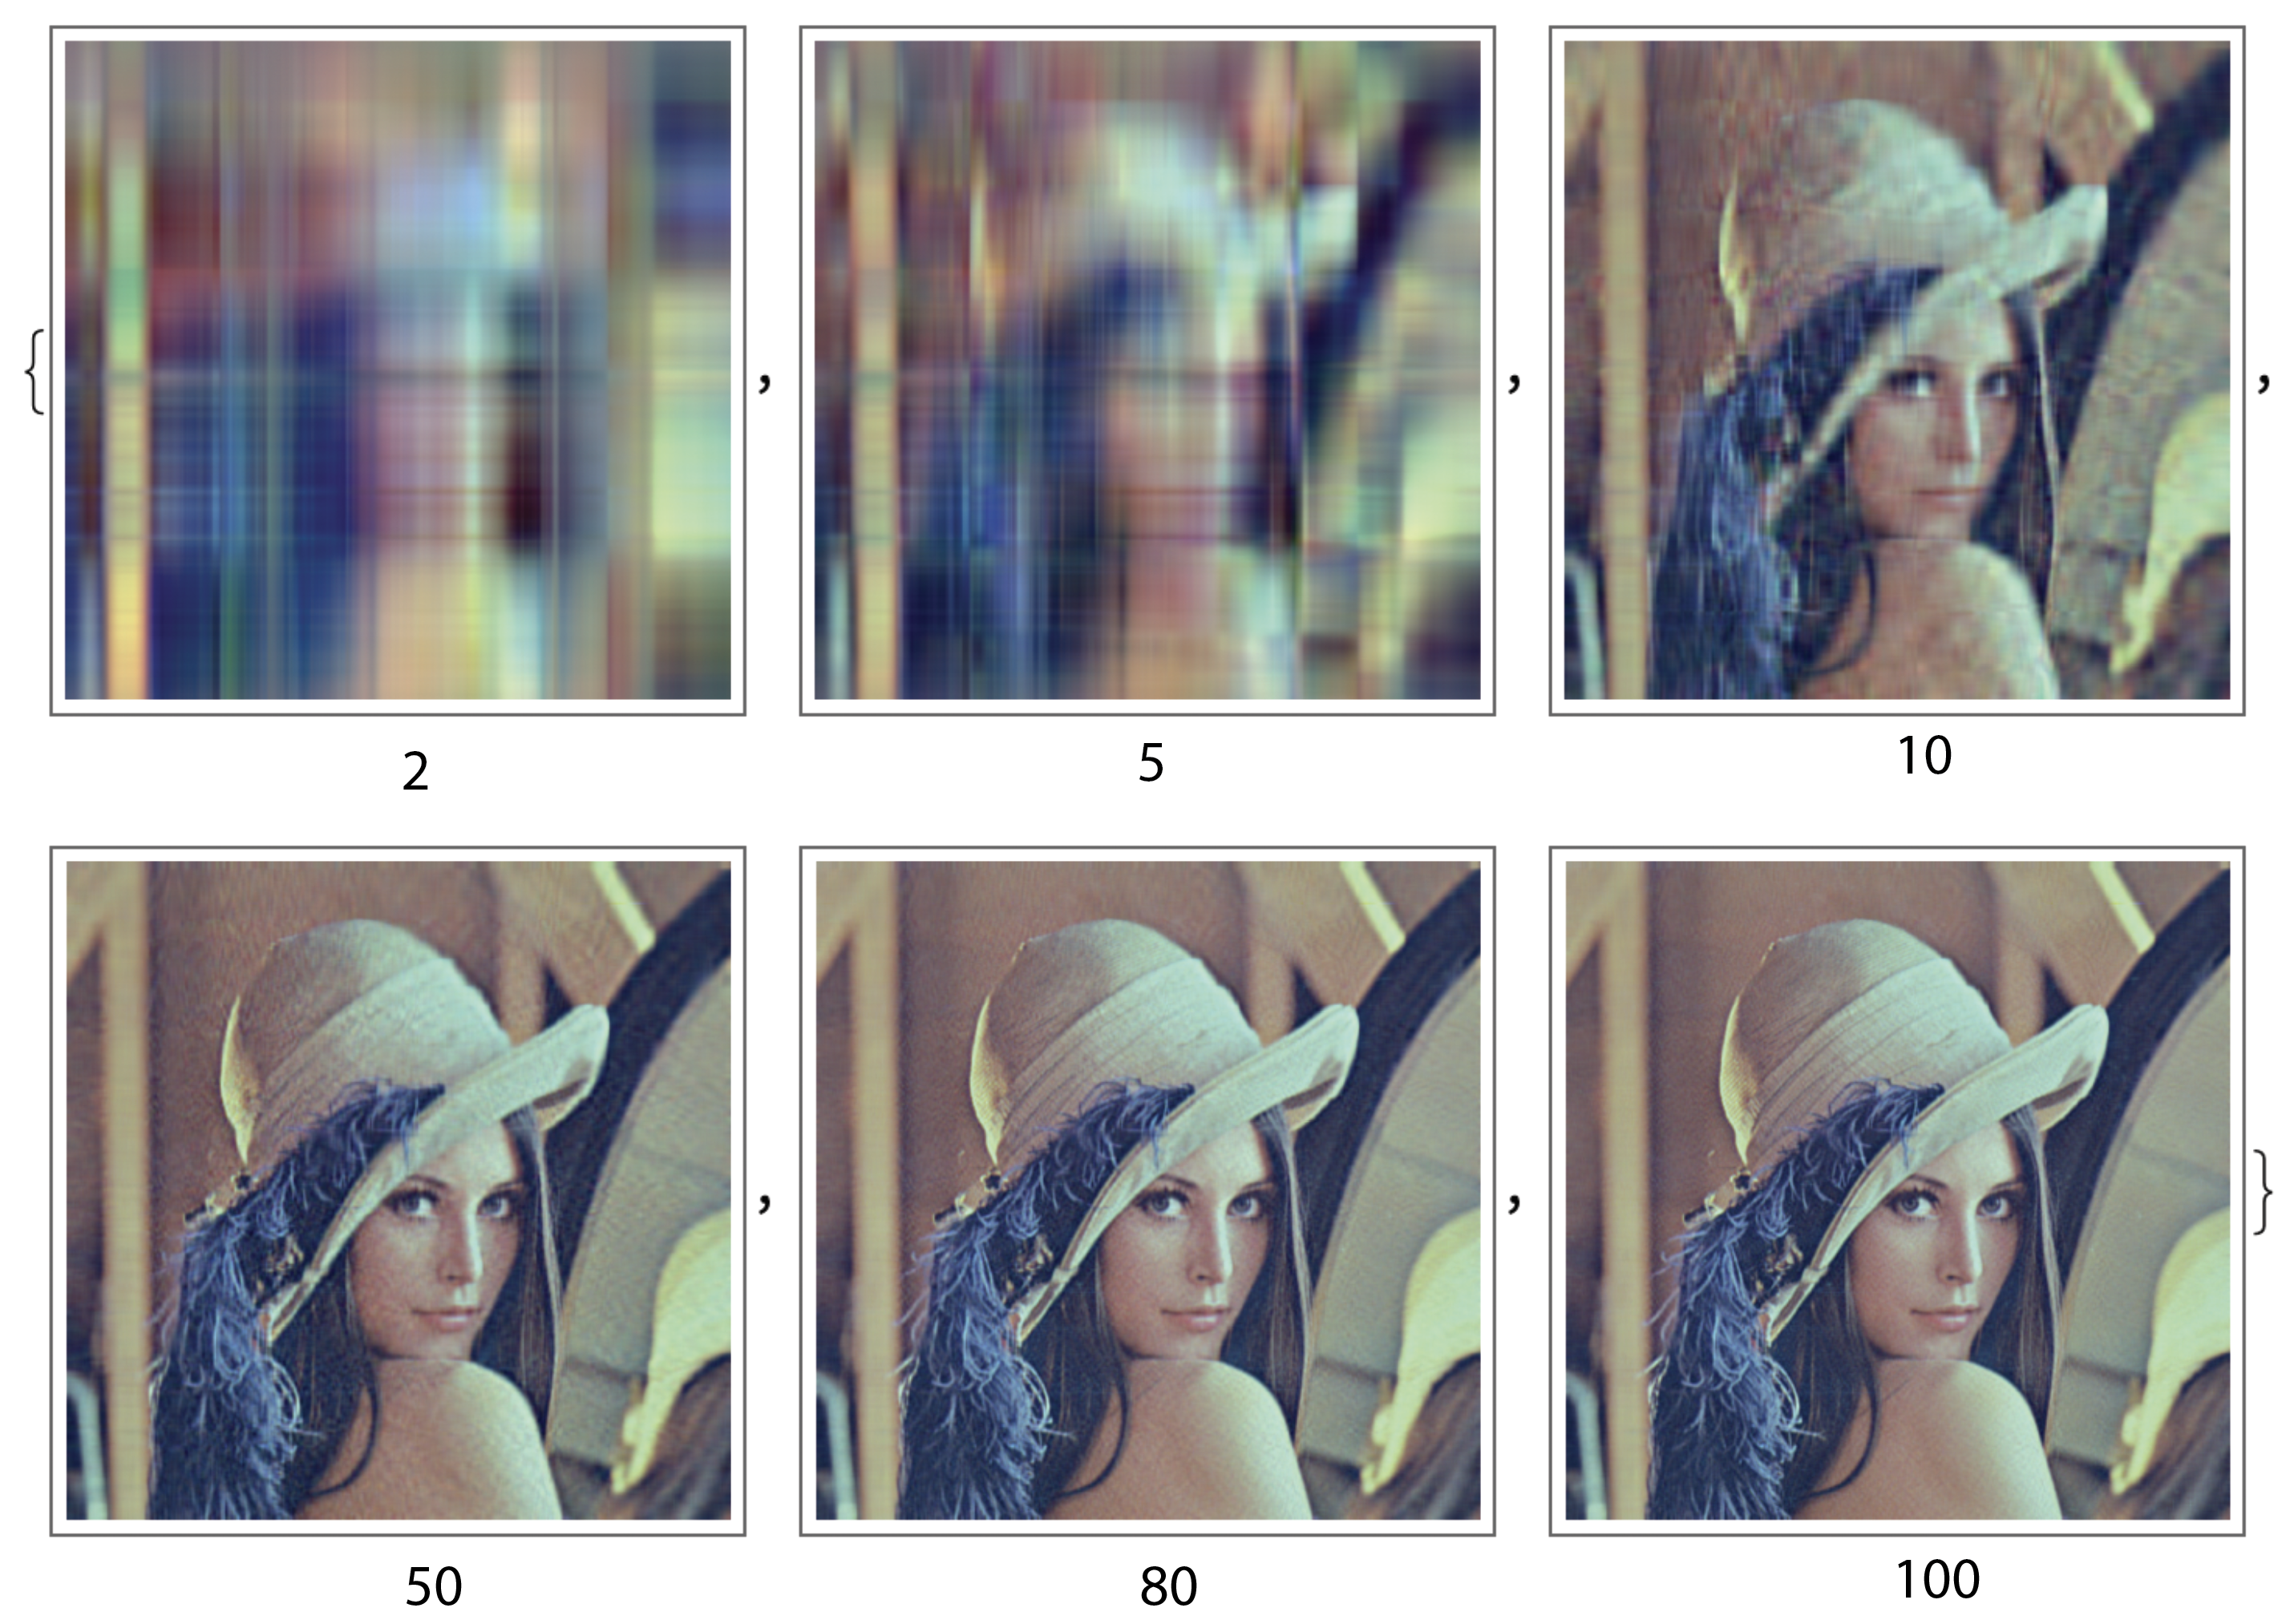
\includegraphics[width=0.6\linewidth]{prob4_recon.png}
		\caption{Reconstructed images using the first $2, 5, 20, 50,80,100$ columns of $\mU$.} % caption of the figure
		\label{fig:fig3}  % Label the figure so you can refer to it in text.
	\end{figure}

	Since PCA uses the principal componants with the largest variances, we can use the variances of each channel in the reconstructed image relative to the original as a measurement of the image quality, i.e. how much of the information (variance) of the original data is retained.
	
	\begin{figure}[H] % This is how figure are placed into latex document
		\centering\includegraphics[width=0.6\linewidth]{prob4_eval.png}
		\caption{Relative variance of the R, G, B channels of reconstructed images with different number of PCs. Each channel is colored by its corresponding color.} % caption of the figure
		\label{fig:fig4}  % Label the figure so you can refer to it in text.
	\end{figure}

	We can see that with 50 PCs, all the 3 channels effectively reach over 90\% of the variance in the original image, and increasing the number of PCs thereafter does not significantly improve image quality. Therefore we can conclude that 50 is the best component number for image reconstruction. 
		\\ \\
	\bold{Codes (Mathematica)}
	\begin{verbatim}
		(*Import picture*)
		
		cwd = NotebookDirectory[];
		original = Import[cwd <> "Lenna_(test_image).png", "Data"];
		pxl = N[Flatten[original, 1]];
		mean = Mean[pxl];
		pxlCtr = # - mean & /@ pxl;
		(*RGB channels*)
		R = ArrayReshape[pxlCtr[[All, 1]], {512, 512}]; G = 
		ArrayReshape[pxlCtr[[All, 2]], {512, 512}]; B = 
		ArrayReshape[pxlCtr[[All, 3]], {512, 512}];
		
		(*PCA and reconstruction*)
		Clear[recon];
		(*Reconstruction single channel*)
		
		recon[channel_, nPC_] := Module[{u, s, v, picrecon},
		(*SVD*){u, s, v} = SingularValueDecomposition[channel];
		(*Reconstruction using nPC columns*)
		picrecon = 
		u[[All, ;; nPC]].s[[;; nPC, ;; nPC]].Transpose[v[[All, ;; nPC]]];
		picrecon]
		(*Reconstruct 3 channels*)
		
		reconRGB[nPC_] := 
		ArrayReshape[
		Transpose[
		Flatten /@ {recon[R, nPC], recon[G, nPC], recon[B, nPC]}], {512, 
			512, 3}]
		rgbPlot[plot_] := 
		ArrayPlot[ArrayReshape[plot, {512, 512, 3}], 
		ColorFunction -> Function[p, RGBColor[p[[1]], p[[2]], p[[3]]]], 
		ColorFunctionScaling -> True]
		
		(*Plotting*)
		rgbPlot[reconRGB[#]] & /@ {2, 5, 20, 50, 80, 100}
		
		(*Evaluation*)
		varPic[picArr_] := N[Variance[ArrayReshape[picArr, {512*512, 3}]]]
		VarOrig = varPic[original];
		percentVar = 
		varPic[reconRGB[#]]/VarOrig & /@ {2, 5, 10, 50, 80, 100};
		ListLinePlot[Transpose[percentVar], 
		Ticks -> {Transpose[{Range[1, 6], {2, 5, 10, 50, 80, 100}}], 
			Automatic}, AxesLabel -> {"Number of PCs", "Variance"}, 
		PlotStyle -> {Red, Green, Blue}, PlotRange -> Full]
	\end{verbatim}
	
	
\end{document}
